\section{Radiation from Continuous Sources III, Electromagnetic Fields in Media}

\subsection{Review}
We have been studying the radiation from a charge/current density:
\begin{equation}
    \begin{split}
        \v{J}(\v{x}, t) &= \v{J}(\v{x})e^{-i\omega t}
        \\ \rho(\v{x}, t) &= \rho(\v{x})e^{-i\omega t}
    \end{split}
\end{equation}
where $\omega = c\frac{2\pi}{\lambda}$ and the current/source is nonzero on length scale $d$. We expanded in $\frac{d}{\lambda} \ll 1$; the leading order approximation is the electric dipole contribution. The first subleading terms came in the form of the magnetic dipole and the electric quadrupole terms. The magnetic dipole fields looked like:
\begin{equation}
    \v{A}(\v{x}) = \frac{ik\mu_0}{4\pi}\hat{\v{n}}\times\v{m}\frac{e^{ikr}}{r}
\end{equation}
with the net magnetic moment defined as the integral of the magnetization density:
\begin{equation}
    \v{m} = \int d^3\v{x}\v{M}(\v{x})
\end{equation}
\begin{equation}
    \v{M}(\v{x}) = \frac{1}{2}\v{x} \times \v{J}
\end{equation}

\subsection{Electric Quadrupole Fields}
We arrived at the magnetic dipole/electric quadrupole term via the symmetric/antisymmetric decomposition:
\begin{equation}
    J^ix'^jn^j = \frac{1}{2}(J^i\hat{\v{n}}\cdot\v{x}' + x'^i\v{J} \cdot \hat{\v{n}}) + \text{a.s.}
\end{equation}
Let's now study the symmetric term appearing above to find the fields from the electric quadrupole:
\begin{equation}\label{eq:quadrupoleintegral}
    \frac{1}{2}\int d^3\v{x}'(\hat{\v{n}}\cdot\v{x}' \v{J} + (\hat{\v{n}}\cdot\v{J})\v{x}')
\end{equation}
Like last class, we can use the continuity equation to manipulate this integral:
\begin{equation}
    i\omega\rho(\v{x}) = \nabla \cdot \v{J}
\end{equation}
wherein the integral of Eq. \eqref{eq:quadrupoleintegral} becomes (after using the continuity equation and integrating by parts):
\begin{equation}
    \frac{1}{2}\int d^3\v{x}'\v{x}'(\hat{\v{n}}\cdot\v{x}')\rho(\v{x}')
\end{equation}
We then get an analogous formula to the (far zone) vector potential as we got for the magnetic dipole:
\begin{equation}
    \v{A}(\v{x}) = \frac{\mu_0 ck^2}{8\pi}\frac{e^{ikr}}{r}\int d^3\v{x}'\v{x}'(\hat{\v{n}}\cdot\v{x}')\rho(\v{x}')
\end{equation}
You can check that this is indeed subleading in $\frac{d}{\lambda}$ (compared to the electric dipole term). Computing the fields:
\begin{equation}
    \v{H} = \frac{ik}{\mu_0}\hat{\v{n}}\times\v{A} = -\frac{ick^3}{8\pi}\frac{e^{ikr}}{r}\int d^3\v{x}'(\hat{\v{n}}\times\v{x}')(\hat{\v{n}}\cdot \v{x}')\rho(\v{x}')
\end{equation}
\begin{equation}\label{eq:quadrapoleE}
    \v{E} = \frac{ik}{\mu_0}Z_0(\hat{\v{n}}\times\v{A})\times\hat{\v{n}}
\end{equation}
Note these have angular dependencies that differ from the electric fields, which you can check in your own time.

\subsection{Moments of a Charge Distribution \& the Quadrupole Tensor/Radiation}
\begin{itemize}
    \item First moment (electric monopole/total charge):
    \begin{equation}
        Q = \int d^3\v{x}\rho(\v{x})
    \end{equation}
    \item Second moment/first subleading moment (electric dipole):
    \begin{equation}
        \v{p} = \int d^3\v{x}\v{x}\rho(\v{x})
    \end{equation}
    which is of particle interest if the total charge is indeed zero, for example for a neutral atom. An example we can consider is the charge distribution sketched below:
    \begin{center}
        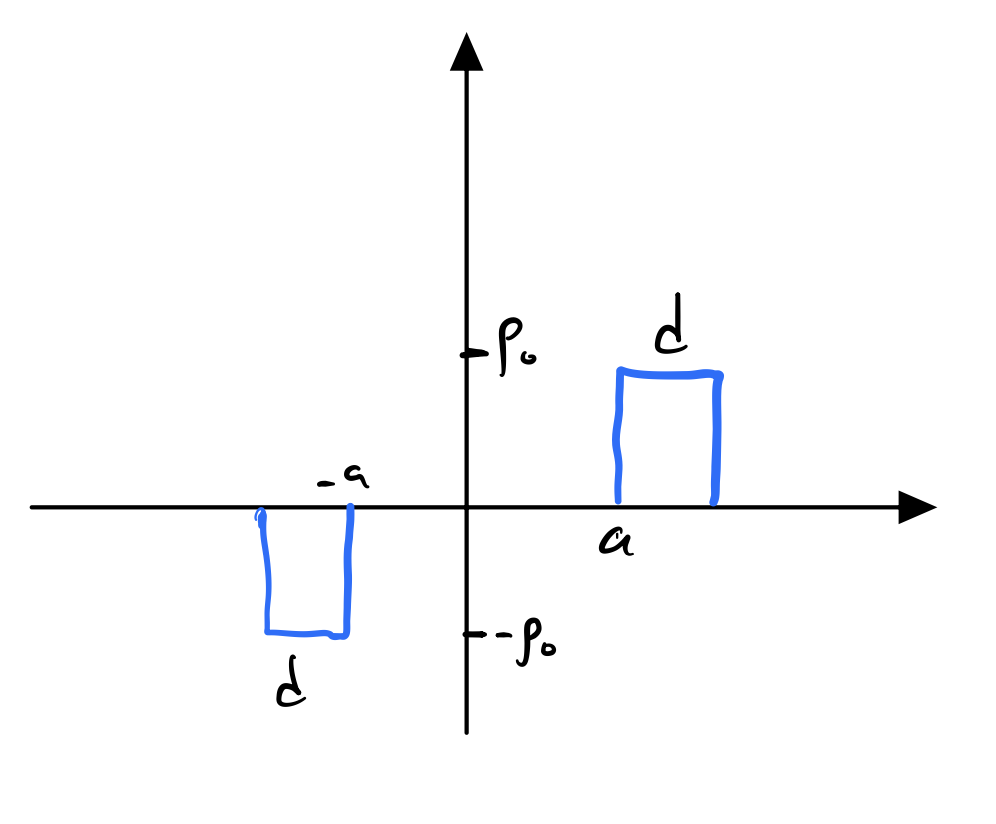
\includegraphics[scale=0.35]{Lectures/Images/lec12-dipoledchargedist.png}
    \end{center}
    where by inspection $Q = 0$, and for the dipole we find:
    \begin{equation}
        p_x = \int_{-\infty}^\infty = x\rho(x) = 2\int_{a}^{a+d}dx x\rho_0 = \rho_0\left[(a + d)^2 - a^2\right]
    \end{equation}
    This is the leading effect of the presence of this charge if we view this distribution from large distances.
    \item Third moment/Second subleading moment (electric quadrupole). Consider the tensor:
    \begin{equation}
        T_{ij} = \int d^3\v{x}x_ix_j\rho(\v{x})
    \end{equation}
    we note that $T_{ij}$ is manifestly symmetric. This has $\frac{3 \cdot 4}{2} = 6$ independent components. This is actually pretty interesting - $T_{ij}$ transforms as 5+1 dimensional object. This just means that the trace is rotationally invariant:
    \begin{equation}
        T_{ii} = \int d^3\v{x}\v{x}^2\rho(\v{x})
    \end{equation}
    the 5 then corresponds to the traceless and symmetric part of the matrix. In the $SU(2)$ language, this is the spin-2 representation (which has $2j + 1$ components), here we deal with $SO(3)$, but they are closely related. The traceless part we can write in the following way:
    \begin{equation}
        Q_{ij} = 3T_{ij} - \delta_{ij}T_{kk}
    \end{equation}
    The claim to fame of this object is that it is traceless:
    \begin{equation}
        Q_{ii} = 3T_{ii} - \delta_{ii}T_{kk} = 3T_{ii} - 3T_{kk} = 0
    \end{equation}
    How does this tensor help us? Going back to our integral that appeared in the quadrapole moment, we could write in index notation:
    \begin{equation}
        -\frac{i\omega}{2}\int d^3\v{x}' x_k'(\hat{n}_lx'_l)\rho(\v{x}')
    \end{equation}
    We can then write:
    \begin{equation}
        x_k'x_l' = \frac{1}{3}(3x_k'x_l' - \delta_{kl}\abs{\v{x}'}^2) + \frac{1}{3}\delta_{kl}\abs{\v{x}'}^2
    \end{equation}
    We note that the $\frac{1}{3}\delta_{kl}\abs{\v{x}'}^2$ term does not contribute to the fields, so we get\footnote{The 24 comes from the fact that famously $24 = 8\times3$}:
    \begin{equation}
        \v{H} = -\frac{ick^3}{24\pi}\frac{e^{ikr}}{r}\hat{\v{n}}\times Q\hat{\v{n}}
    \end{equation}
    where $Q$ is the 3x3 traceless symmetrix matrix $Q_{ij}$, and:
    \begin{equation}
        Q\hat{\v{n}} = Q_{ij}n_j
    \end{equation}
    We can then calculate the electric field $\v{E}$ from Eq. \eqref{eq:quadrapoleE}, and then from this calculate the differential power\footnote{I won't do the factorization of 1152 for you...}:
    \begin{equation}
        \dod{P}{\Omega} = \frac{c^2Z_0}{1152\pi^2}k^6\abs{(\hat{\v{n}} \times Q\hat{\v{n}}) \times \hat{\v{n}}}^2
    \end{equation}
    This tells us how much radiation is associated with the quadrapole moment of the distribution. If we integrate over all angles:
    \begin{equation}
        P = \frac{c^2Z_0k^6}{1440\pi}\sum_{ij}^3\abs{Q_{ij}}^2
    \end{equation}
    this goes as $k^6$, while the dipole contribution goes as $k^4$. This is exactly as we expect - with each higher order moment we get one more power of $\frac{d}{\lambda}$ ($k$ - the $d$ is hiding in the moment) and hence in the power with each moment we get two more powers of $k$.
\end{itemize}

\subsection{Review - Electrostatics in Media}
Now we move back to Wald (Chapter 6) and discuss electrodynamics in media, e.g. the study of light waves propagating in water.
Last quarter you looked at electrostatics in media, but now we look at what changes in the dynamical case. But, since its been a while since you've had this discussion, let us review. 

Suppose we were in a non-vacuous media\footnote{I suppose air is technically a non-vacuous medium... certainly less violent than if the room was filled with honey. It would be quite difficult to breathe.}.There, there are notions of free charges and currents, as well as dipoles that may react to external fields and polarize the substance. It is also useful to average over a distance $L$ (not worry about the microscopics of the medium). Suppose $\psi$ is any physical quantity. We can then define the average as:
\begin{equation}
    \avg{\psi}(\v{x}) = \int d^3\v{x}' \psi(\v{x}')f_l(\v{x} - \v{x}')
\end{equation}
where $f_l(\v{x} - \v{x}')$ is a function that starts at 1 and drops off smoothly/quickly at length scale $L$.

\begin{center}
    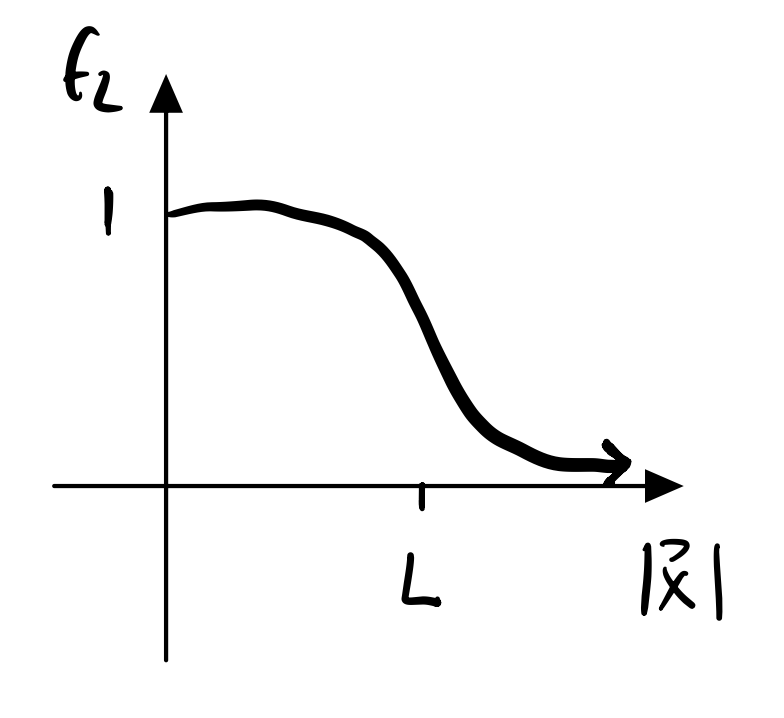
\includegraphics[scale=0.35]{Lectures/Images/lec12-fL.png}
\end{center}

We can look at the $\v{D}$-field in vacuum:
\begin{equation}
    \v{D}_{\text{vac}} = \e_0\v{E}_{\text{vac}}
\end{equation}
which we can average, anticipating that in matter we will want to coarse grain:
\begin{equation}
    \avg{\v{D}_{\text{vac}}} = \e_0\avg{\v{E}_{\text{vac}}}
\end{equation}
in matter we further add a polarization term:
\begin{equation}
    \avg{\v{D}} = \e_0\avg{\v{E}} + \avg{\v{P}}
\end{equation}
and there is an analogous expression for the $\v{H}$-field:
\begin{equation}
    \avg{\v{H}} = \frac{1}{\mu_0}\avg{\v{B}} - \avg{\v{M}}
\end{equation}

\subsection{Modifying Maxwell's Equations}
The first question we may ask is how we may modify Maxwell's equation now that we are inside a medium. The first thing to say is that Maxwell's equations are always true - so let's just start by writing them down again:
\begin{equation}\label{eq:Gauss}
    \nabla \cdot \v{E} = \frac{\rho}{\e_0}
\end{equation}
\begin{equation}\label{eq:Ampere}
    \nabla \times \v{B} - \frac{1}{c^2}\dot{\v{E}} = \mu_0 \v{J}
\end{equation}
\begin{equation}\label{eq:magneticGauss}
    \nabla \cdot \v{B} = 0
\end{equation}
\begin{equation}\label{eq:Faraday}
    \nabla \times \v{E} + \dot{\v{B}} = 0
\end{equation}
as we discussed when we studied the relativistically covariant version of the Maxwell equations, the source-free/Bianchi identity equations (Eqs. \eqref{eq:magneticGauss}, \eqref{eq:Faraday}) just become their averaged versions:
\begin{equation}
    \nabla \cdot \avg{\v{B}} = 0
\end{equation}
\begin{equation}
    \nabla \times \avg{\v{E}} + \avg{\dot{\v{B}}} = 0
\end{equation}
and further we remember from our discussion of electrostatics that Eq. \eqref{eq:Gauss} can be modified to be:
\begin{equation}
    \nabla \cdot \avg{\v{D}} = \avg{\rho_f}
\end{equation}
with $\rho_f$ the free charge density. The last equation Eq. \eqref{eq:Ampere} requires a little more consideration. Last quarter you saw that:
\begin{equation}
    \avg{J} \stackrel{\text{static}}{=} \avg{\v{J}_f} + \nabla \times \avg{\v{M}}
\end{equation}
but this is modified now to include a time derivative of the polarization:
\begin{equation}
    \avg{J} = \avg{\v{J}_f} + \nabla \times \avg{\v{M}} + \dpd{}{t}\avg{\v{P}}
\end{equation}
then combining this with:
\begin{equation}
    \avg{\v{H}} = \frac{1}{\mu_0}\avg{\v{B}} - \avg{\v{M}}
\end{equation}
we find the equivalent of Eq. \eqref{eq:Ampere}:
\begin{equation}
    \nabla \times \avg{\v{H}} - \dpd{}{t}\avg{\v{D}} = \avg{\v{J}_f}
\end{equation}
note the presence of the new $\p_t \avg{\v{D}}$ term! this was not important last quarter in electrostatics, but it is something we must consider here.

The situation is quite a bit subtle in the dynamic case. In the static case for example, there is no ambiguity about what are free charges - free charges are what can move in the presence of an external electric field, while the bound charges are those that do not move. So there is no mystery about what $\rho_f$ is. But here it is not obvious what $\rho_f$ is - how do we think about an electron that stays in the metal (but moves) in the presence of a sinusoidal field; is it free or bound? Really the issue is whether the microscopic charges contribute to $\rho_f$ or to the polarization $\v{P}$ (and a similar story with $\v{J}_f$ and $\v{M}$). There is an ambiguity, and we have to make sure we do not double count the contributions. This whole speech was to say that we need to break this ambiguity somehow - here we will take $\v{P}$ seriously.

Note that $\v{P}, \v{E}$ are not independent, and indeed the polarization depends on the electric field. Let us work in the limit where:
\begin{equation}
    \avg{\v{P}} \propto \avg{\v{E}}
\end{equation}
and so:
\begin{equation}
    \avg{\v{D}} = \e \avg{\v{E}}
\end{equation}
and similarly:
\begin{equation}
    \avg{\v{H}} = \frac{1}{\mu}\avg{\v{B}}
\end{equation}
What are $\e, \mu$? They are features of the material that we must measure. We will focus on how to modify this discussion in the dynamical case. What we've assumed - $\avg{\v{P}(t)} \propto \avg{\v{E}(t)}$ - doesn't quite make sense because it implies that the polarization at time $t$ reacts to the electric field at the same time $t$ instantaneously. For now, let us pretend it is correct in the sense that the variation of the electric field in time is slow (and so the material has time to react). Thus Maxwell's equations (with sources) can be written as:
\begin{equation}
    \nabla \cdot \avg{\v{E}} = \frac{1}{\e}\avg{\rho_f}
\end{equation}
\begin{equation}
    \nabla \times \avg{\v{B}} - \mu \e \avg{\dot{\v{E}}} = \mu\avg{\v{J}_f}
\end{equation}
These equations look the same as the equations in vacuum, just that we have replaced fields with their averages and have replaced $\e_0, \mu_0 \to \e, \mu$. We can define the index of refraction:
\begin{equation}
    n = \frac{\sqrt{\e\mu}}{\sqrt{\e_0\mu_0}}
\end{equation}
and if we go to the discussion in Wald chapter 5 and replace all $\e_0, \mu_0, c, \rho, \phi_f \to \e, \mu, c/n, \avg{\rho_f}, \avg{\phi_f}$, we will find EM waves propagating with speed $c/n$. In a little more detail, we can define a ``Lorenz gauge'':
\begin{equation}
    \frac{n^2}{c^2}\avg{\dot{\phi}} + \nabla \cdot \avg{\v{A}} = 0
\end{equation}
where in this gauge:
\begin{equation}
    \tilde{\square}\avg{\phi} = -\frac{1}{c}\avg{\rho_f}
\end{equation}
\begin{equation}
    \tilde{\square}\avg{\v{A}} = -\mu\avg{\v{J}_f}
\end{equation}
and:
\begin{equation}
    \tilde{\square} = -\frac{n^2}{c^2}\dpd[2]{}{t} + \nabla^2
\end{equation}
where $\frac{n^2}{c^2} = \frac{1}{c_{\text{mat}}^2}$.

A couple more comments - suppose the material we consider was infinite in extension. Then the waves propagate forever in the material. But any real material of course has a boundary. 

\begin{center}
    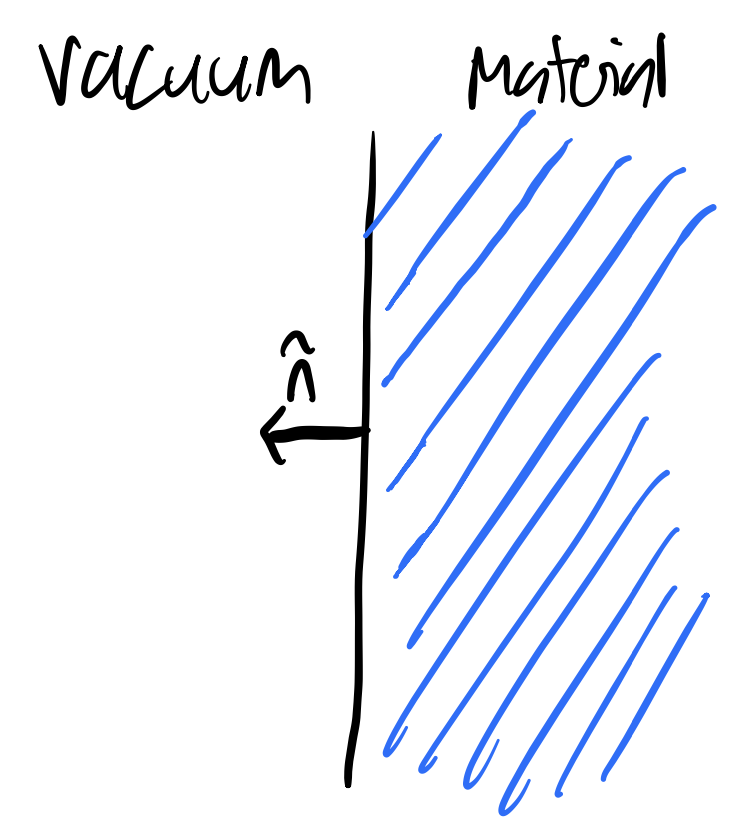
\includegraphics[scale=0.35]{Lectures/Images/lec12-interface.png}
\end{center}

We then have the boundary conditions:
\begin{itemize}
    \item $\avg{E_\parallel}, \hat{\v{n}}\cdot\avg{\v{B}}$ are continuous
    \item If there are no $\delta$-function contributions to $\avg{\rho_f}, \avg{\v{J}_f}$, then $\hat{\v{n}}\cdot\avg{\v{D}}, \avg{H_\parallel}$ are continuous.
\end{itemize}
Next week, you will study this scenario, and derive Snell's law on your problem set.